%%%%%%%%%%%%%%%%%%%%%%%%%%%%%%%%%%%%%%%%%%%%%%%%%%%%%%%%%%%%%%%%%%%%%%%%%%%%%%%%%%%%%%%%%%%%%%%%%%%%%%%%%%%%%%%%%%%%%%%%%%%%%%%%%%%%%%%%%%

% 此文档是复旦数本科毕业论文的标准模板,首次使用前请先阅读README文档.

% 请使用xelatex对模板进行编译,若想引用参考文献也能正确显示,请依次按照xelatex->bibtex->xelatax->xelatex进行编译.

% by 杨闻浩 2024-3
%%%%%%%%%%%%%%%%%%%%%%%%%%%%%%%%%%%%%%%%%%%%%%%%%%%%%%%%%%%%%%%%%%%%%%%%%%%%%%%%%%%%%%%%%%%%%%%%%%%%%%%%%%%%%%%%%%%%%%%%%%%%%%%%%%%%%%%%%%
\documentclass[a4paper,punct=banjiao,twoside]{ctexrep}
% documentclass 可选择 ctexart, ctexrep, ctexbook.
% oneside/twoside 单面/双面打印适配版本.
% openright/openany 控制新的章节是否应该在奇数页的右侧开始, 但并不好用,建议手动插入空白页.
% fontset 设置字体集,可以选择的值包括 windows、mac、ubuntu 等,可以解决字体报错.
% punct=: 设置中文文档中的标点样式,可选的值包括 quanjiao 全角式:所有标点占一个汉字宽度,相邻两个标点占 1.5 汉字宽度;banjiao 半角式:所有标点占半个汉字宽度;kaiming 开明式:句末点号16用占一个汉字宽度,标号和句内点号占半个汉字宽度;等.


\usepackage[a4paper,hmargin={2.54cm,2.54cm},vmargin={3.175cm,3.175cm}]{geometry}
\headheight = 15 pt
%参见https://tex.stackexchange.com/questions/132170/what-do-headheight-headsep-etc-do-in-the-vmargin-package最高赞答案

\usepackage{amsmath,amssymb}
% 扩展支持的数学符号

\usepackage{mathrsfs}
% 引用


\usepackage[dvipsnames, svgnames, x11names]{xcolor}
% 扩展颜色

\usepackage[colorlinks=true,linkcolor=Maroon]{hyperref}
% 使用hyperref宏包, 对目录, 公式引用, 文献引用做超链接, 超链接方便电子版的阅读, 但不影响打印.
% pdfborder对超链接的边框大小进行设置, 模板中默认边框大小为0.
% colorlinks=true, 表示超链接对应的文字采用超链接边框的颜色, =false时保持原字体颜色.
% linkcolor=maroon, 设置超链接边框的颜色, 可以改为red,green等等.

\usepackage{amsthm}
% 配置定理环境
\theoremstyle{plain}
%plain(默认样式): 定理名称是正体,定理内容是斜体.
%definition: 定理名称和定理内容都是正体,其上下留有额外的空间.
%remark: 正体,其上下没有额外的空间.
\newtheorem{thm}{定理}[chapter]
% 如果需要在每一节中单独编号,请将[chapter]改为[section]
\newtheorem{lemma}[thm]{引理}
\newtheorem{axiom}[thm]{公理}
\newtheorem{coro}[thm]{推论}
\newtheorem{prop}[thm]{命题}
\newtheorem{con}[thm]{猜想}

\theoremstyle{definition}
\newtheorem{defn}[thm]{定义}
\newtheorem{asm}[thm]{假设}
\newtheorem{que}[thm]{问题}

\theoremstyle{remark}
\newtheorem{rem}{注}[chapter]
\newtheorem{example}{例}[chapter]
% 除了注和例之外,均是连续编号.

\renewcommand{\proofname}{\textbf{证明}}

% 如需将证毕符号改成黑色的正方形,请将下一行取消注释.
% \renewcommand{\qedsymbol}{$\blacksquare$}    


\newcommand{\dd}{\text{d}}
\newcommand{\R}{{\mathbb R}}
\newcommand{\N}{{\mathbb N}}
%\newcommand{\Z}{{\mathbb Z}}
%\newcommand{\C}{{\mathbb C}}
% 此处可以定义一些常用的记号,留给大家自由发挥咯,例如输入\dd 可以直接得到正体的d,用作积分号里dx中的d.

%其余的一些必要的宏包
\usepackage{xcolor,caption,array,enumerate}

\usepackage{graphicx} %插入图片的宏包
\usepackage{float} %设置图片浮动位置的宏包
\usepackage{subcaption} %插入多图时用子图显示的宏包

\usepackage{tikz}%画图

\usepackage{longtable, booktabs, threeparttable, caption, bicaption, multirow}
% 扩展表格功能

\usepackage[ruled,linesnumbered]{algorithm2e}
% 算法

\usepackage{listings}
\lstset{
  language=Python, % 设置语言
  basicstyle=\ttfamily, % 设置字体族
  breaklines=true, % 自动换行
  keywordstyle=\bfseries\color{NavyBlue}, % 设置关键字为粗体,颜色为 NavyBlue
  morekeywords={}, % 设置更多的关键字,用逗号分隔
  emph={self}, % 指定强调词,如果有多个,用逗号隔开
  emphstyle=\bfseries\color{Rhodamine}, % 强调词样式设置
  commentstyle=\itshape\color{black!50!white}, % 设置注释样式,斜体,浅灰色
  stringstyle=\bfseries\color{PineGreen!90!black}, % 设置字符串样式
  columns=flexible,
  numbers=left, % 显示行号在左边
  numbersep=2em, % 设置行号的具体位置
  numberstyle=\footnotesize, % 缩小行号
  frame=single, % 边框
  framesep=1em % 设置代码与边框的距离
}

% 自定义多级标题格式
\CTEXsetup[nameformat={\huge \heiti},titleformat={\huge \heiti},beforeskip={0.0cm},afterskip={1.2cm}]{chapter}
% 上一行为旧版的语法,可以选择注释上一行,取消注释下一行.
%\ctexset { chapter = { nameformat={\huge \heiti  },titleformat={\huge \heiti  },beforeskip={0.0cm},afterskip={1.2cm} } } 
\usepackage{titlesec}
\titleformat{\section}[block]{\Large\centering\heiti\bfseries}{\arabic{chapter}.\arabic{section}}{1em}{}[]
\titleformat{\subsection}[block]{\large \heiti\bfseries}{\arabic{chapter}.\arabic{section}.\arabic{subsection}}{1em}{}[]
\titleformat{\subsubsection}[block]{\normalsize\bfseries}{\arabic{subsection}-\alph{subsubsection}}{1em}{}[]
\titleformat{\paragraph}[block]{\small\bfseries}{[\arabic{paragraph}]}{1em}{}[]
% 使用Ctex自带的\section的标题会出现问题,使用titlesec\chapter的标题要么无法显示汉字数字,要么无法显示字母A,只能做缝合怪了!

\usepackage{gbt7714}
% 将参考文献的格式更改为与国标《文后参考文献著录规则》GB/T 7714-2005一致.
% 需要使用其它格式时请将该行注释, 并在参考文献部分将指定语句取消注释.


%导言区设置完毕
%%%%%%%%%%%%%%%%%%%%%%%%%%%%%%%%%%%%%%%%%%%%%%%%%%%%%%%%%%%%%%%%%%%%%%%%%%%%%%%%%%%%%%%%%%%%%%%%%%%%%%%%%%%%%%%%%%%%%%%%%%%%%%%%%%%%%%%%%%
\begin{document}
% 制作封面, 适用于研究生毕业论文.
%\begin{titlepage}
%    {
%        \hfill 
%        \footnotesize
%    \begin{tabular}{cc}
%        \makebox[4em][s]{学校代码}:&\makebox[5em][l]{10246}\\
%        \makebox[4em][s]{学号}:&\makebox[5em][l]{??300180???}\\
%
%    \end{tabular}
%    }
%    \vspace*{1.5cm}
%
%    \begin{center}
%        \begin{figure}[H] %H为当前位置,!htb为忽略美学标准,htbp为浮动图形
%            \centering %图片居中
%            
\includegraphics[width=0.46\textwidth]{figs/fudan-name.pdf} %插入图片,[]中设置图片大小,{}中是图片文件名
%            %\caption{Main name 0} %最终文档中希望显示的图片标题
%            \label{fudan-name} %用于文内引用的标签
%        \end{figure}
%        \vspace*{1.5cm}
%
%        \makebox[16em][s]{\LARGE{本科毕业论文}}
%        %(学术学位)
%        %若需要取消注释上一行,请相应改变下一行的行间距的取值
%        \vspace*{3cm}
%
%        {\bfseries \Large 论文题目}
%        \vspace*{1cm}
%
%        {\bfseries  English Title}
%        \vspace*{3cm}
%
%        \fontsize{14pt}{\baselineskip}\selectfont
%        \begin{tabular}{cc}
%            \makebox[6em][s]{院系}:&\makebox[8em][c]{数学科学学院}\\[1ex]
%            \makebox[6em][s]{专业}:&\makebox[8em][c]{数学与应用数学}\\[1ex]
%            \makebox[6em][s]{姓名}:&\makebox[8em][c]{XXX}\\[1ex]
%            %两个字姓名的同学可以将上一行改为
%            %\makebox[6em][s]{姓名}:&\makebox[3em][c]{XX}\\[1ex]
%            \makebox[6em][s]{指导老师}:&\makebox[8em][c]{XXX \ 教授}\\[1ex]
%            \makebox[6em][s]{完成日期}:&\makebox[8em][c]{\today}\\[1ex]
%        \end{tabular}     
%    \end{center}
%\end{titlepage}

\renewcommand{\thepage}{\roman{page}}

% 改写目录标题的格式
\renewcommand{\contentsname}{目\quad 录}
\tableofcontents
\setcounter{page}{1}

\chapter*{摘\quad 要}
\addcontentsline{toc}{chapter}{摘要}
\normalsize

这是我的中文摘要.

\chapter*{Abstract}
\addcontentsline{toc}{chapter}{Abstract}
\normalsize

This is my English abstract.

\noindent{\textbf{Keywords:}} 1; 2; 3\\
\noindent{\textbf{CLC code:}} O24

\clearpage
\mbox{}
\thispagestyle{empty}
% 为了保证第一章在奇书页.

\renewcommand{\thepage}{\arabic{page}}
\setcounter{page}{0}
% 论文的页码从正文重新开始计数

\chapter{数学语言}

\section{数学符号和公式}

\begin{itemize}
    \item 公式应另起一行居中排版.公式后应注明编号, 按章顺序编排, 编号右端对齐.
    \item 公式末尾是需要添加标点符号的, 至于用逗号, 句号还是不加, 取决于公式下面一句是接着公式说的, 还是另起一句.
    \begin{equation}
  \frac{2h}{\pi}\int_{0}^{\infty}\frac{\sin\left( \omega\delta \right)}{\omega}
  \cos\left( \omega x \right) \mathrm{d}\omega = 
  \begin{cases}
    h, & \left| x \right| < \delta, \\
    \frac{h}{2}, & x = \pm \delta, \\
    0, & \left| x \right| > \delta.
  \end{cases}
\end{equation}
    \item 公式较长时最好在等号“$=$”处转行.
    \begin{align}
    & I (X_3; X_4) - I (X_3; X_4 \mid X_1) - I (X_3; X_4 \mid X_2) \nonumber \\
  = & [I (X_3; X_4) - I (X_3; X_4 \mid X_1)] - I (X_3; X_4 \mid \tilde{X}_2) \\
  = & I (X_1; X_3; X_4) - I (X_3; X_4 \mid \tilde{X}_2).
\end{align}
\item 公式较长时最好在等号“$=$”处转行.
如果在等号处转行难以实现, 也可在 $+$、$-$、$\times$、$\div$ 运算符号处转行, 转行
时运算符号仅书写于转行式前, 不重复书写.
\begin{multline}
  \frac{1}{2} \Delta (f_{ij} f^{ij}) =
    2 \left(\sum_{i<j} \chi_{ij}(\sigma_{i} - \sigma_{j})^{2}
    + f^{ij} \nabla_{j} \nabla_{i} (\Delta f) \right. \\
  \left. + \nabla_{k} f_{ij} \nabla^{k} f^{ij} +
    f^{ij} f^{k} \left[2\nabla_{i}R_{jk}
    - \nabla_{k} R_{ij} \right] \vphantom{\sum_{i<j}} \right).
\end{multline}
\end{itemize}


\section{定理环境}

这里举一个“定义”和“定理”的例子.

\begin{defn}[非负整指数索伯列夫空间\cite{ChenPDE}]
设$\Omega\subset\mathbb{R}^n$是一个给定区域,令$m$为非负整数,$1\leq p\leq \infty$.定义索伯列夫空间$W^{m,p}$为
$$
W^{m,p}(\Omega)=\left\{u\in L^p(\Omega): \text{对任意}\alpha\in \mathbb{N}_{0}^n\text{满足 }0\leq |\alpha|\leq m, D^{\alpha}u\in L^p(\Omega) \right\},
$$
并装备以范数
\begin{equation*}
\begin{aligned}
\|u\|_{W^{m,p}(\Omega)} &= \left( \sum_{|\alpha|\leq m} \|D^{\alpha}u\|_{L^p(\Omega)}^p \right)^{1/p},\quad 1\leq p <\infty, \label{eq:sobolev-norm}\\
\|u\|_{W^{m,\infty}(\Omega)} &= \max_{|\alpha|\leq m} \|D^{\alpha}u\|_{L^{\infty}(\Omega)}.
\end{aligned}
\end{equation*}
\end{defn}


\begin{thm}[索伯列夫嵌入定理{\cite{AF03}}]\label{thm:sobolev-embedding}
令$\Omega$为$\mathbb{R}^n$上一个有$C^{\infty}$光滑边界的有界区域.令$j\geq 0, m\geq 1$为整数, $1\leq p<\infty$, 如下嵌入关系成立:
\begin{enumerate}
\item 如果$mp>n>(m-1)p$,则
$$
W^{m,p}(\Omega) \hookrightarrow C^{0,s}(\overline{\Omega}), \quad \text{对于 }0<s\leq m-\frac{n}{p}.
$$
如果$n=(m-1)p$,则
$$
W^{m.p}(\Omega) \hookrightarrow C^{0,s}(\overline{\Omega}), \quad \text{对于 }0<s<1.
$$
\item 如果$1\leq k\leq n$,以及$mp=n$,则
$$
W^{j+m,p}(\Omega)\hookrightarrow W^{j,q}(\Omega), \quad \text{对于 }p\leq q < \infty.
$$
\item 如果$mp<n$,则
$$
W^{j+m,p}(\Omega) \hookrightarrow W^{j,q}(\Omega), \quad \text{对于 }p\leq q \leq p^{*}:=\frac{np}{n-mp}.
$$
\end{enumerate}
\end{thm}



\section{线性方程的适定性理论}\label{sec:linear-wellposedness}
本节摘自邹森博士的毕业论文, 包含一些数学符号的使用、定理的叙述与证明、数学式的引用.

在这一节中, 我们讨论线性薛定谔方程
\begin{equation}\label{eq:schrodinger-0}
\left\{\begin{aligned}
-\Delta u - k^2 u +c(x)u &=F, && x\in\Omega,\\
u &=f, && x\in\partial\Omega
\end{aligned}\right.
\end{equation}
弱解的适定性, 从而定义反问题的观测数据DtN算子. 此外, 为研究非线性方程的适定性, 我们使用了线性亥姆霍兹方程
\begin{equation}\label{eqn:Helmholtz}
\left\{\begin{aligned}
-\Delta u - k^2 u &=F, && x\in\Omega,\\
u &=f, && x\in\partial\Omega
\end{aligned}\right.
\end{equation}
的强解理论, 我们也在本节中加以介绍.这些结论都可以从一般形式椭圆方程的弱解和强解理论导出.为简洁起见, 我们首先给出如下定义:我们定义散度型微分算子为
\begin{equation}\label{eq:divergence-form}
L:=-\sum_{i=1}^n D_i(a^{ij}(x)D_{j})+c(x).
\end{equation}
称散度型微分算子$L$在区域$\Omega$上满足椭圆性条件,如果对于任意$x\in\Omega$,$\xi\in\mathbb{R}^n$,存在常数$\lambda,\Lambda>0$,使得
\begin{equation}\label{eq:strict-elliptic}
\lambda |\xi|^2 \leq \sum_{i,j=1}^n a^{ij}(x)\xi_{i}\xi_{j} \leq \Lambda|\xi|^2 .
\end{equation}
另外我们定义非散度型微分算子
\begin{equation}\label{eq:nondivergence-form}
L=-\sum_{i,j=1}^{n}a^{ij}(x)D_{ij} + c(x).
\end{equation}
类似地, 对于非散度型微分算子, 我们也可以定义其椭圆性条件:对于任意$x\in\Omega$,$\xi\in\mathbb{R}^n$,存在常数$\lambda,\Lambda>0$,使得
\begin{equation*}
\lambda |\xi|^2 \leq \sum_{i,j=1}^n a^{ij}(x)\xi_{i}\xi_{j} \leq \Lambda|\xi|^2 .
\end{equation*}
对于以上两种形式的微分算子, 在后文的讨论中, 除非特殊说明, 我们假定对于$1\leq i,j\leq n$,有$a^{ij}(x)\in C^{\infty}(\overline{\Omega})$以及$c\in L^{\infty}(\Omega)$.

\subsection{弱解的存在性和连续依赖性}\label{sec:weak-solution}

我们首先叙述一般形式椭圆方程的Dirichlet问题弱解的存在性:
\begin{thm}[Dirichlet问题弱解的存在性{\cite{Chen2elliptic}}]\label{thm:weak-solution}
令$L$为\eqref{eq:divergence-form}中定义的散度型椭圆微分算子,令$\Omega\subset\mathbb{R}^n$为有界开区域,使得Sobolev嵌入定理在其上成立.对于$\mu\in\mathbb{R}$,Dirichlet问题
\begin{equation}\label{eq:dirichlet-equation}
\left\{\begin{aligned}
& Lu+\mu u = F,\\
& u-g\in H_0^1(\Omega)\end{aligned}\right.
\end{equation}
的解有两种情况:
\begin{enumerate}[(1)]
\item 对任意$F\in H^{-1}(\Omega)$,$g\in H^{1}(\Omega)$,\eqref{eq:dirichlet-equation}存在唯一弱解$u\in H^1(\Omega)$;
\item 存在一个非平凡的$u\in H^1_0(\Omega)$使得$Lu+\mu u=0$.
\end{enumerate}
更进一步,满足情形(2)的全体$\mu$构成的集合为可数离散的,$\infty$是唯一可能的极限点,我们称这样的$\mu$为$L$算子在$\Omega$上的Dirichlet特征值,记为$\operatorname{Spec}_{\Omega}(L)$,或者简写为$\operatorname{Spec}(L)$.对于每一Dirichlet特征值$\mu$,其对应的特征函数空间是有限维的.
\end{thm}

如果增加$c\geq 0$几乎处处成立的假设条件,有如下结论:
\begin{thm}[Dirichlet问题的$H^1$弱解{\cite{Chen2elliptic}}]\label{thm:regularity}
令$L$为\eqref{eq:divergence-form}中定义的散度型椭圆微分算子,令$\Omega\subset\mathbb{R}^n$为有界开区域,使得其上成立索伯列夫嵌入定理.进一步假设$c\geq 0$几乎处处成立.对于任意$F\in H^{-1}(\Omega)$和$g\in H^1(\Omega)$, Dirichlet问题
\begin{equation}
\left\{\begin{aligned}
&Lu = F, \\
& u-g\in H^{1}_{0}(\Omega)
\end{aligned}\right.
\end{equation}
存在唯一弱解,而且满足估计式
\begin{equation}
\|u\|_{H^1_0(\Omega)} \leq C\left(\|F\|_{H^{-1}(\Omega)} +\|g\|_{H^1(\Omega)} \right),
\end{equation}
其中常数$C$与$F$和$g$无关.
\end{thm}

在\eqref{eq:schrodinger-0}中我们仅假设$c\in L^{\infty}(\Omega)$,不满足定理\ref{thm:regularity}中$c\geq 0$几乎处处成立的条件,但是通过避开特征值的假设,我们依然可以利用定理\ref{thm:weak-solution}和定理\ref{thm:regularity}得到\eqref{eq:schrodinger-0}弱解的适定性结论:
\begin{coro}[线性薛定谔方程\eqref{eq:schrodinger-0}的适定性]\label{cor:Schrodinger-weak-solution}
令$\Omega\subset\mathbb{R}^n$为带$C^1$边界的有界开区域.如果$k^2$不是$-\Delta+c$在$\Omega$上的Dirichlet特征值,则对于任意$F\in H^{-1}(\Omega)$, $f\in H^{1/2}(\partial\Omega)$, Dirichlet问题\eqref{eq:schrodinger-0}存在唯一解$u\in H^1(\Omega)$,且满足估计式
\begin{equation}\label{eq:regularity-weak-solution}
\|u\|_{H^1(\Omega)} \leq C\left(\|F\|_{H^{-1}(\Omega)} +\|f\|_{H^{1/2}(\partial\Omega)} \right),
\end{equation}
其中常数$C$仅仅依赖于$k,c$和$\Omega$.
\end{coro}
注意到当$c(x)\equiv 0$时,上述推论依然成立,因此我们也可以得到\eqref{eqn:Helmholtz}的适定性.

\begin{proof}
根据定理\ref{thm:weak-solution},由于$k^2$不是$-\Delta+c$在$\Omega$上的Dirichlet特征值,故我们可以得到$u$的存在唯一性.现在我们证明弱解$u$满足\eqref{eq:regularity-weak-solution}.不失一般性,我们只考虑齐次边界条件$f=0$的情形.

由于$c\in L^{\infty}(\Omega)$,故存在常数$s\in\mathbb{R}$,使得$c(x)+s\leq 0$对于$x\in\Omega$几乎处处成立.我们记$L:=-\Delta +c$,$L_{s}=-\Delta +s +c$.令定理\ref{thm:regularity}中$g\equiv 0$,我们可以得到$L_{s}$为$H_{0}^1(\Omega)\rightarrow H^{-1}(\Omega)$的有界线性算子,且存在连续的逆算子$L_{s}^{-1}:H^{-1}(\Omega)\rightarrow H^{1}_0(\Omega)$.对于$s$使得$k^2+s\ne 0$,我们记$\sigma=(k^2+s)^{-1}$,则对于$u\in H^{1}_0(\Omega)$有如下等价形式
\begin{equation}\label{eq:eu0}
Lu=k^2 u +F \quad \Leftrightarrow \quad L_{s} u = (k^2+s)j\circ i(u) + F
\quad \Leftrightarrow \quad (\sigma I-K)(i(u)) = \sigma i L_s^{-1}F
\end{equation}
其中$i: H^{1}_0(\Omega)\rightarrow L^2(\Omega)$, $j:L^2(\Omega)\rightarrow H^{-1}(\Omega)$为自然的包含映射, $K:=i\circ L_s^{-1} \circ j$.

由于我们假设$k^2\notin\operatorname{Spec}(-\Delta+c)$,根据定理\ref{thm:regularity}的证明过程,$K$为紧自伴算子{\cite{Chen2elliptic}}.故我们可以取得$s$使得$\sigma\notin\operatorname{Spec}(K)$,此时$\sigma I-K$为$L^2(\Omega)\rightarrow L^2(\Omega)$的可逆线性算子.也就是说,对于任意$F\in H^{-1}(\Omega)$,存在$\tilde{u}\in L^2(\Omega)$,使得
\begin{equation}\label{eq:eu1}
(\sigma I-K)\tilde{u} = \sigma i L_s^{-1}F.
\end{equation}
结合\eqref{eq:eu0}和\eqref{eq:eu1}我们可以得出存在$u\in H^{1}_0(\Omega)$使得$\tilde{u}=i(u)$.根据定理\ref{thm:regularity}以及$\sigma I-K$和$L_{s}$的可逆性,我们有
\begin{equation*}
\begin{aligned}
\|u\|_{H^1(\Omega)} &\leq C\left( \left\|(k^2+s) j(\tilde{u})\right\|_{H^{-1}(\Omega)} + \|F\|_{H^{-1}(\Omega)} \right)\\
&\leq C\left( \|\tilde{u}\|_{L^2(\Omega)} + \|F\|_{H^{-1}(\Omega)} \right)\\
& \leq C\left( \left\|\sigma(\sigma I-K)^{-1}\circ i\circ L^{-1}_s F\right\|_{L^2(\Omega)} + \|F\|_{H^{-1}(\Omega)} \right)\\
& \leq C\|F\|_{H^{-1}(\Omega)}.
\end{aligned}
\end{equation*}

对于非齐次边界条件的情况,即$f\ne 0$,我们可以对$w=u-Ef$应用以上过程得到\eqref{eq:regularity-weak-solution},其中$E$为$\operatorname{Tr}:H^{1}(\Omega)\rightarrow H^{1/2}(\partial\Omega)$的右逆算子.
\end{proof}

\chapter{图表}
\section{插图}
插图功能是利用TeX的特定编译程序提供的机制实现的,不同的编译程序支持不同的图形方式. XeTeX支持插入 EPS、PDF、PNG、JPEG 格式的图片.一般图形都是处在浮动环境中.之所以称为浮动是指最终排版效果图形的位置不一定与源文
件中的位置对应.如果要强制固定浮动图形的位置,请使用float宏包,它提供了 \texttt{[H]} 参数.

\subsection{单个图形}
\begin{figure}[H]
    \begin{center}
        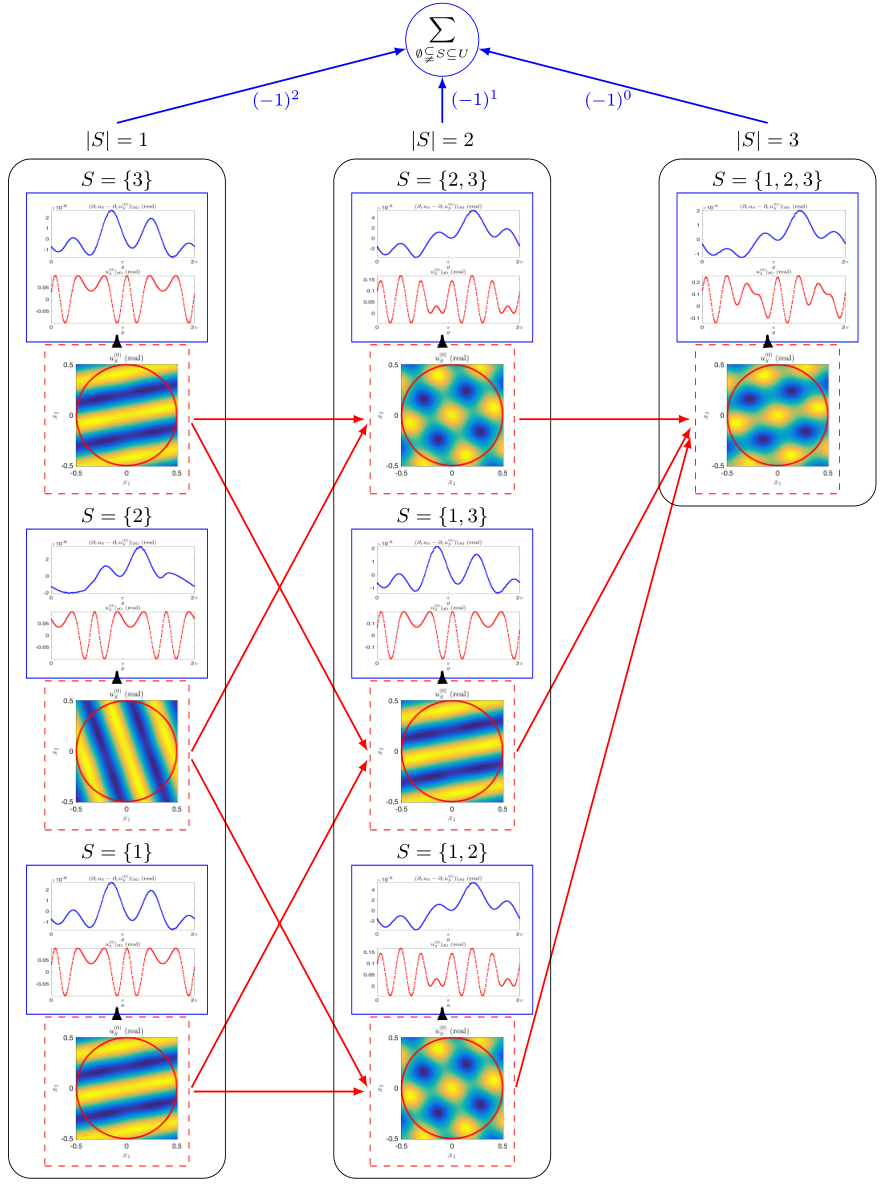
\includegraphics[width=0.5\textwidth]{./figs/cost.png}
\caption[Alessandrini-PIE等式与组合解$u_{S}^{(0)}$]{在非线性次数$m=3$和波数$k=15$时,组合解$u_{S}^{(0)}$的生成.\textbf{红色矩形(虚线)}:$|\xi| = 45.6$时的组合解$u_{S}^{(0)}$.
\textbf{蓝色矩形(实线):} Dirichlet边值 $u_{S}^{(0)} \big|_{\partial\Omega}$ (\textcolor{red}{红色曲线})和线性化Neumann数据的近似$\big( \partial_{\nu} u_{S} - \partial_{\nu} u_{S}^{(0)} \big) \big|_{\partial\Omega}$ (\textcolor{blue}{蓝色曲线}).
\textbf{蓝色圆圈}:根据Alessandrini-PIE等式做组合.}
\label{fig:superposition}
\end{center}
\end{figure}

\subsection{多个图形}
\begin{figure}[H]
\centering
\textbf{非线性次数} $m = 5$ \\[1ex]
\,\hfill \textbf{(i)} $k = 5$ \hfill\,\\
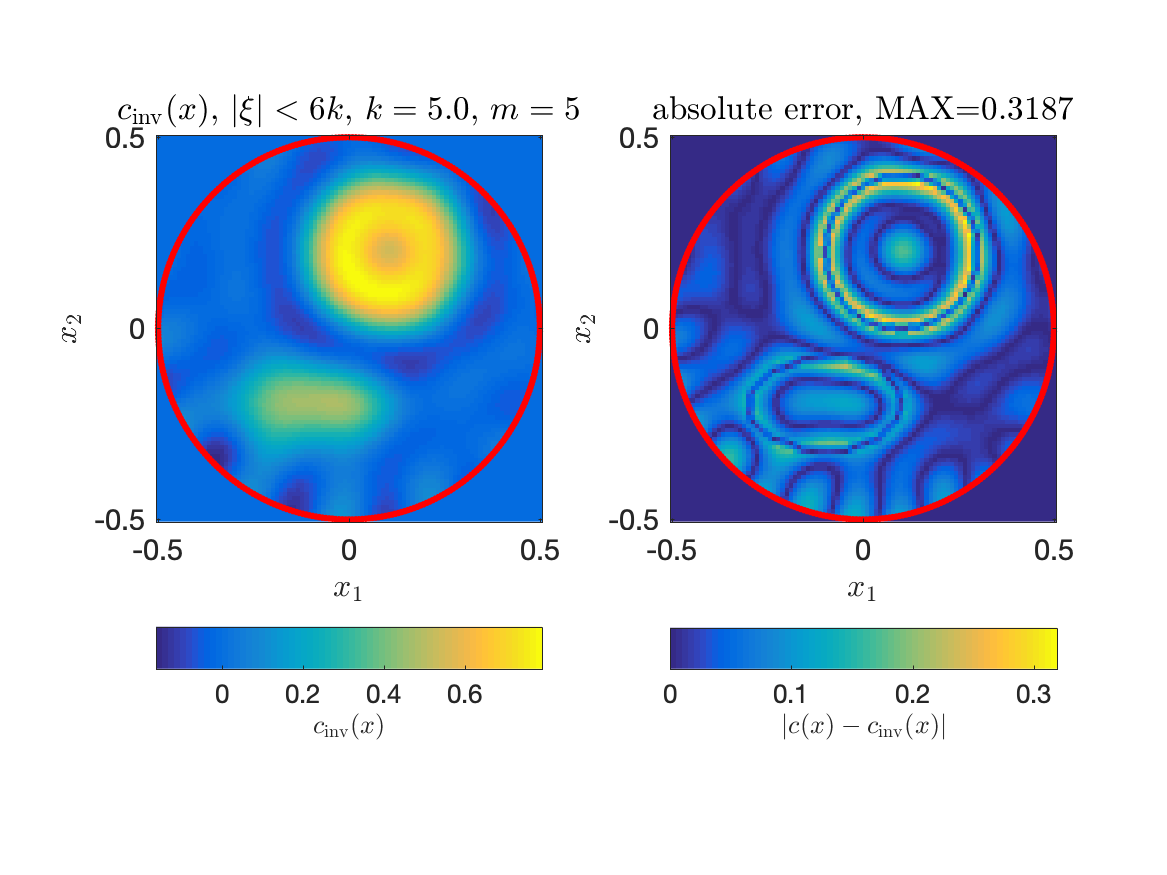
\includegraphics[width=0.45\textwidth,trim=20 60 20 35,clip]{./figs/pwc_5_Ic_0050.png}
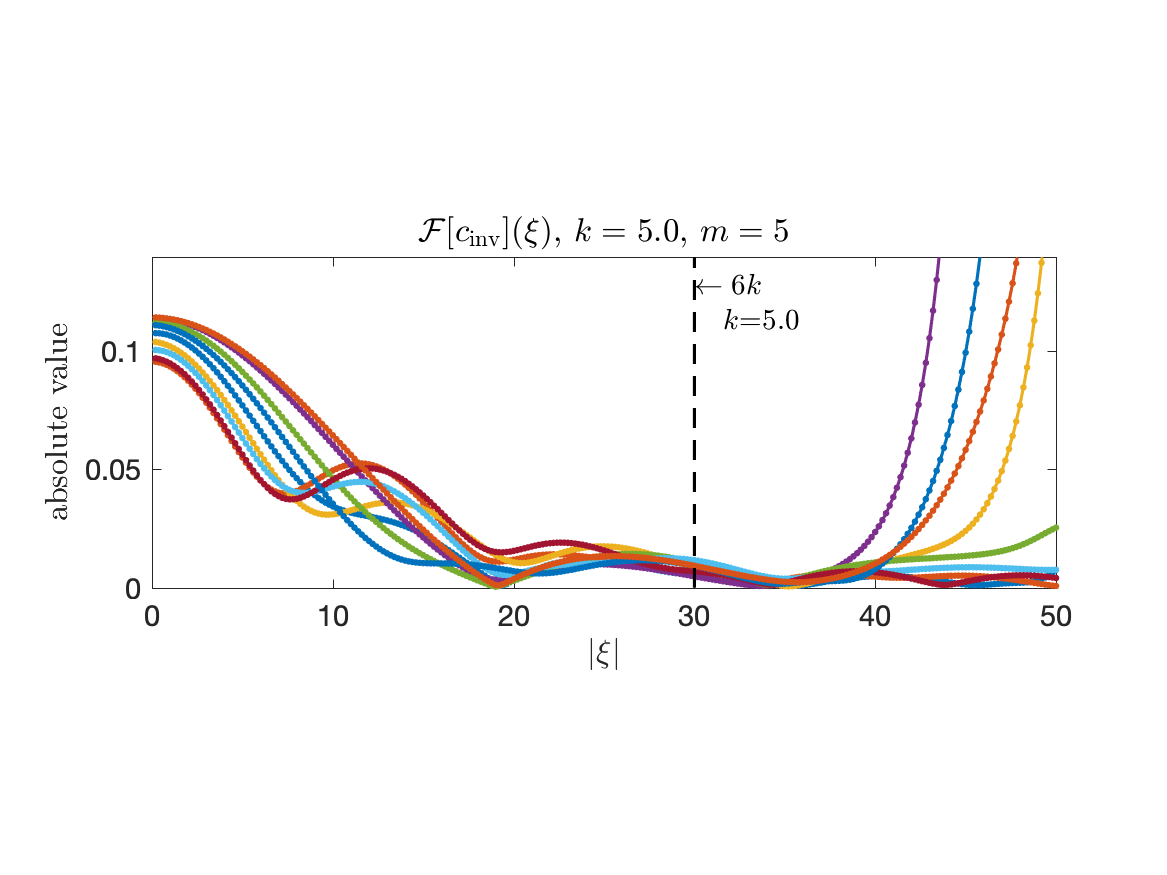
\includegraphics[width=0.54\textwidth,trim=10 60 30 90,clip]{./figs/pwc_5_Fc_0050.png}\\
\,\hfill \textbf{(i)} $k = 10$ \hfill\,\\
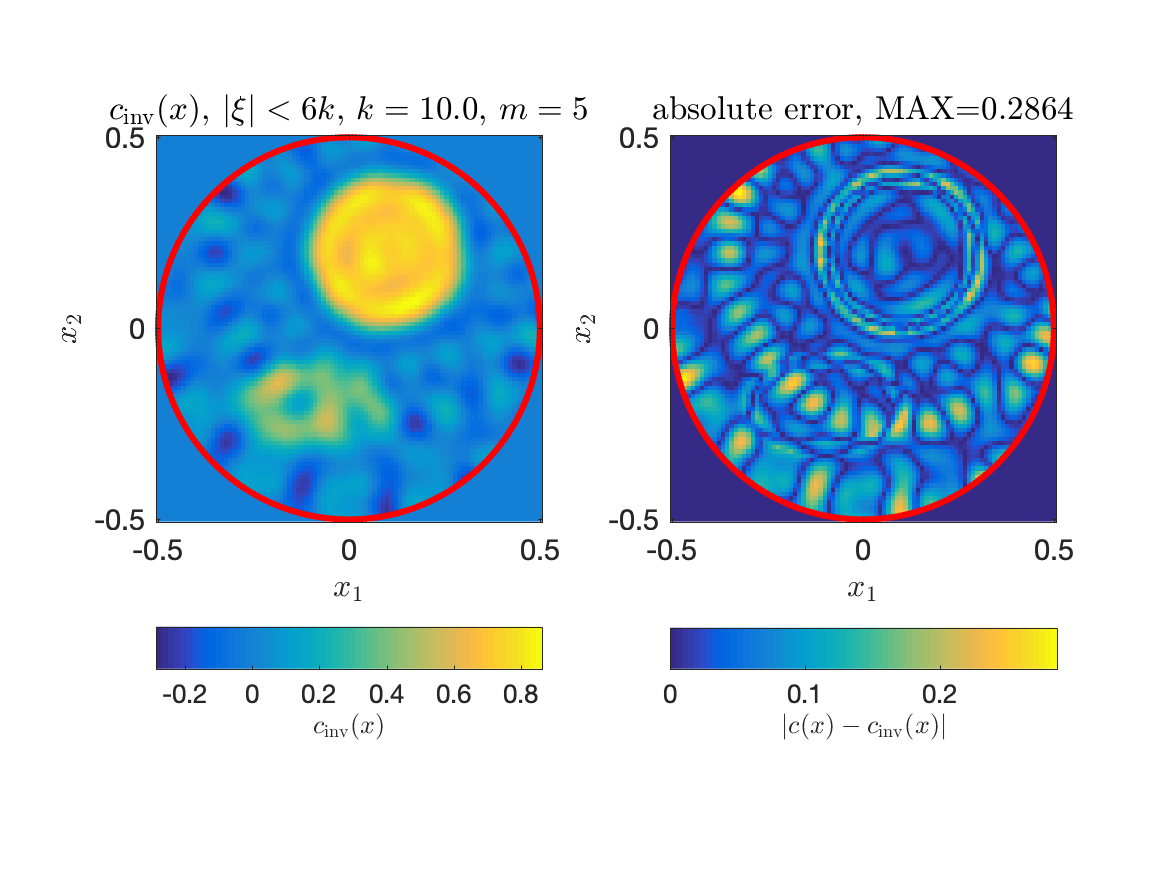
\includegraphics[width=0.45\textwidth,trim=20 60 20 35,clip]{./figs/pwc_5_Ic_0100.png}
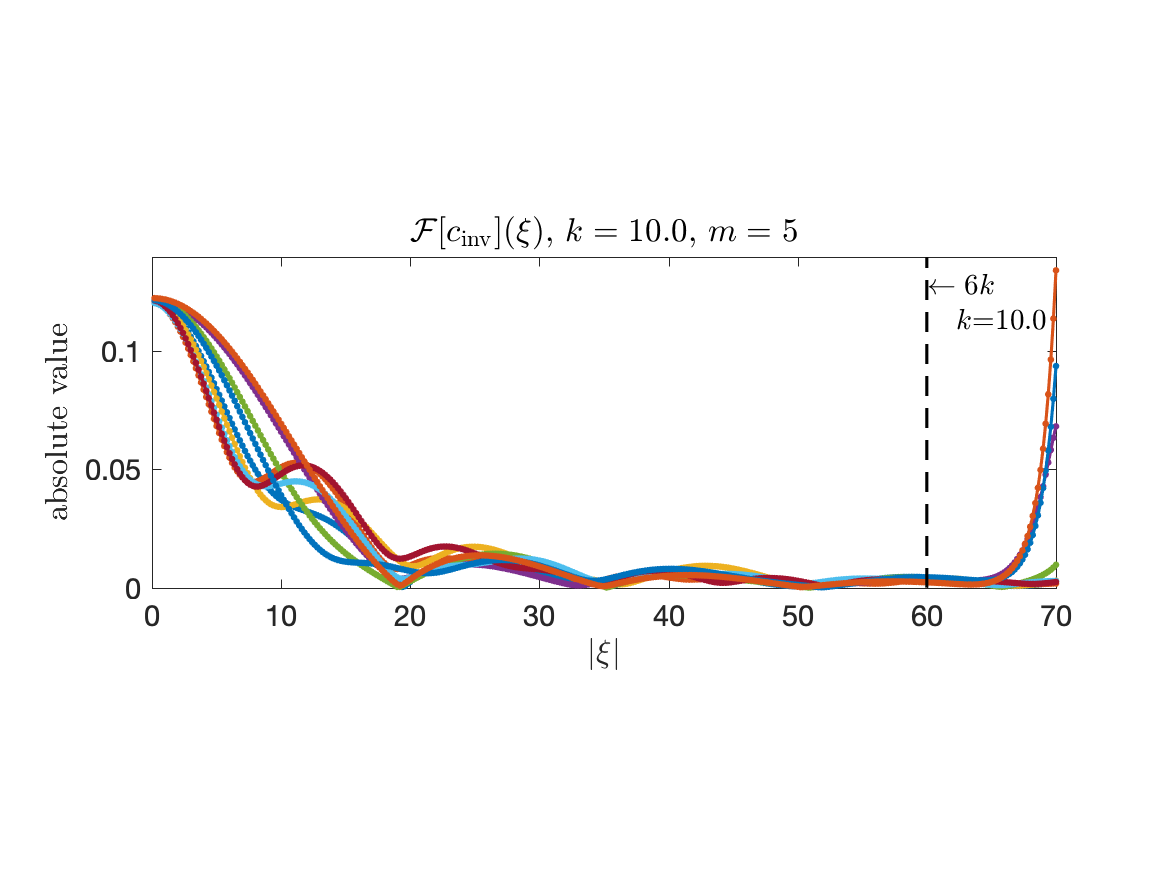
\includegraphics[width=0.54\textwidth,trim=10 60 30 90,clip]{./figs/pwc_5_Fc_0100.png}\\
\,\hfill \textbf{(i)} $k = 15$ \hfill\,\\
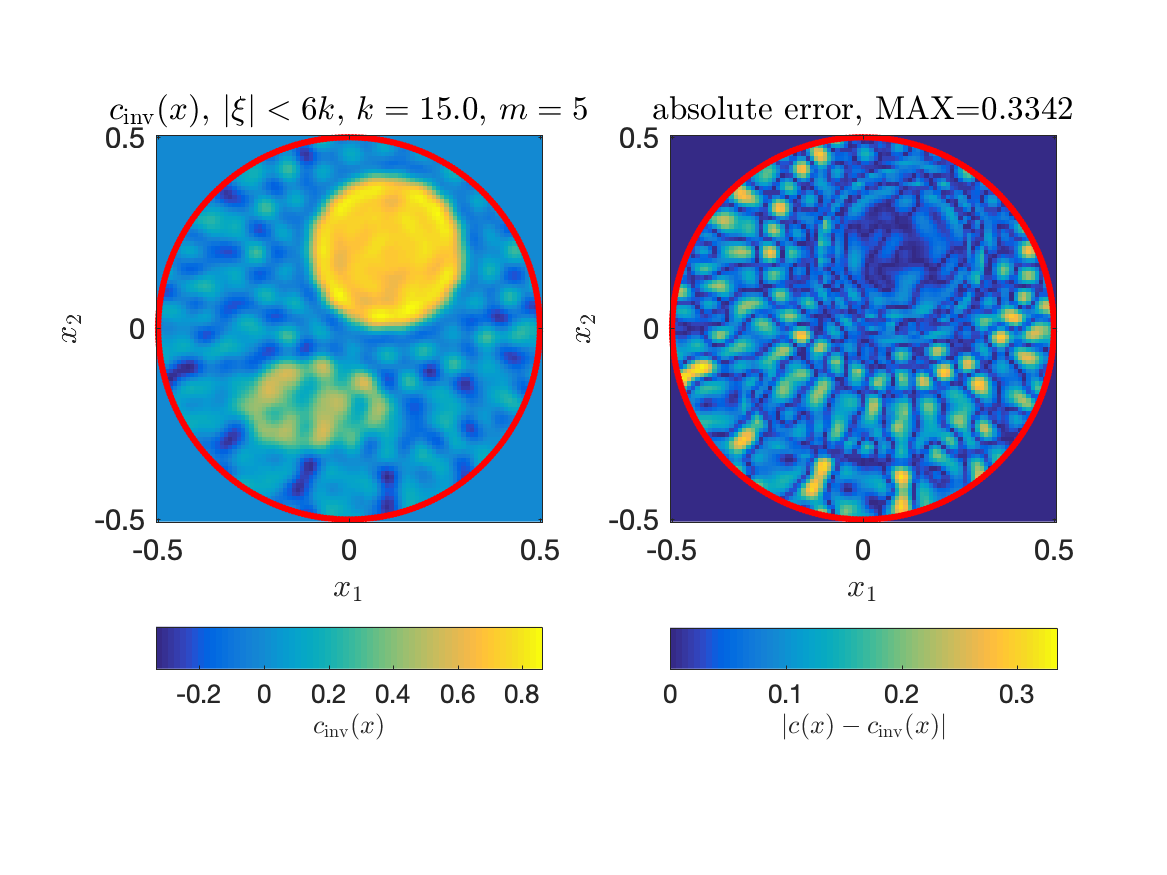
\includegraphics[width=0.45\textwidth,trim=20 60 20 35,clip]{./figs/pwc_5_Ic_0150.png}
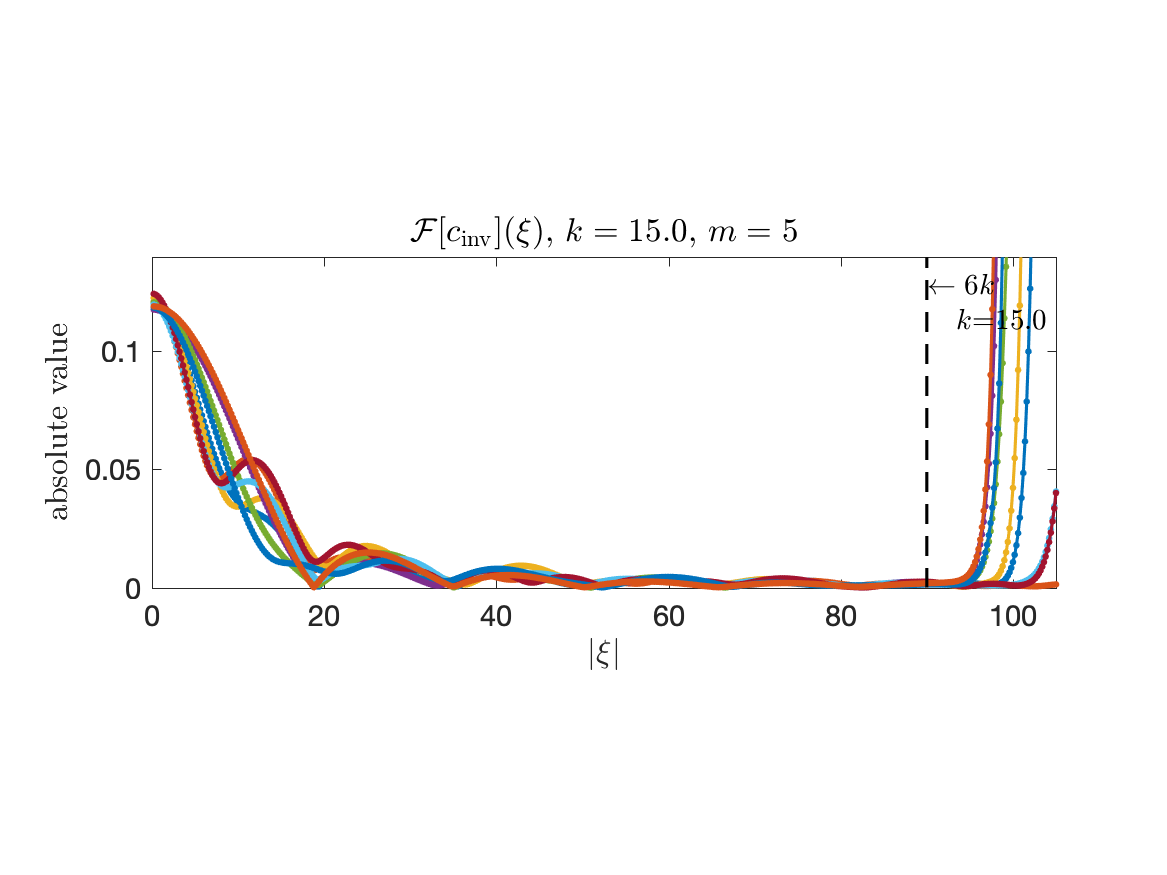
\includegraphics[width=0.54\textwidth,trim=10 60 30 90,clip]{./figs/pwc_5_Fc_0150.png}\\
\caption[算法2:不连续位势的重构结果]{当非线性次数$m=5$,波数\textbf{(i)} $k = 5$,\textbf{(ii)} $k = 10$和\textbf{(iii)} $k = 15$时的重构结果.
第一列:利用频域截断$|\xi| \leq (m+1)k$得到的重构位势函数$c_{\textrm{inv}}(x)$.
第二列:真实位势函数和重构位势函数的角度误差$|c(x) - c_{\textrm{inv}}(x)|$.
第三列:重构位势函数的傅立叶系数的绝对值$\mathcal{F}[c_{\textrm{inv}}](\xi)|$.
}
\label{fig:5_pwc}
\end{figure}

如果多个图形相互独立,并不共用一个图形计数器,那么用 \texttt{minipage} 或者
\texttt{parbox} 就可以,如图~\ref{fig:parallel1} 与图~\ref{fig:parallel2}.

\begin{figure}[H]
  \centering
  \begin{minipage}{0.48\textwidth}
    \centering
    
\includegraphics[height=1.5cm]{./figs/fudan-emblem.pdf}
    \caption{并排第一个图}
    \label{fig:parallel1}
  \end{minipage}\hfill
  \begin{minipage}{0.48\textwidth}
    \centering
    
\includegraphics[height=1.5cm]{./figs/fudan-emblem.pdf}
    \caption{并排第二个图}
    \label{fig:parallel2}
  \end{minipage}
\end{figure}

如果要为共用一个计数器的多个子图添加子图题,建议使用较新的 subcaption 宏包,不建议使用 subfigure 或 subfig 等宏包.

推荐使用 subcaption宏包的 subcaptionbox并排子图,子图题置于子图之下,子图号用 a)、b) 等表示.也可以使用subcaption宏包的 subcaption(放在 minipage中,用法同 caption).

subcaption 宏包也提供了subfigure和 subtable 环境,如
图~\ref{fig:subfigure}.

\begin{figure}[!htp]
  \centering
  \begin{subfigure}{0.3\textwidth}
    \centering
    
\includegraphics[height=2cm]{./figs/fudan-emblem.pdf}
    \caption{校徽}
  \end{subfigure}
  \hspace{1cm}
  \begin{subfigure}{0.4\textwidth}
    \centering
    
\includegraphics[height=1.5cm]{./figs/fudan-emblem.pdf}
    \caption{校徽.这个图略矮些,subfigure中同一行的子图在顶端对齐.}
  \end{subfigure}
  \caption{包含子图题的范例(使用 subfigure)}
  \label{fig:subfigure}
\end{figure}

\subsection{Tik作图}
以下摘自Hansimov的知乎文章[LaTeX 绘图指南 - 001] TikZ 的简介、资源以及学习方法\footnote{\href{https://zhuanlan.zhihu.com/p/48300815}{https://zhuanlan.zhihu.com/p/48300815}}.

TikZ 是 LaTeX 下的一个(著名的)绘图宏包.TikZ 的德文原文是 TikZ ist kein Zeichenprogramm, 这是一个 "GNU's Not Unix!" 式的递归缩写.翻译成英文就是 TikZ is not a drawing program,中文意思是“TikZ 不是一个绘图程序”. (程序员式冷幽默)

PGF/TikZ 相关的学习资源很多,可以参考这个项目:xiaohanyu/awesome-tikz\footnote{\href{https://github.com/xiaohanyu/awesome-tikz}{https://github.com/xiaohanyu/awesome-tikz}}.基本列出了常见的高质资源,语言大多为英文.此外还有一些重要的资源:

\begin{itemize}
    \item 英文文档:pgfmanual\footnote{\href{http://mirrors.ctan.org/graphics/pgf/base/doc/pgfmanual.pdf}{http://mirrors.ctan.org/graphics/pgf/base/doc/pgfmanual.pdf}}
    \item PGF/TikZ 中文手册(在翻):pgfmanual-zh\footnote{\href{https://github.com/Hansimov/pgfmanual-zh}{https://github.com/Hansimov/pgfmanual-zh}}
    \item 命令大全:VisualTikZ\footnote{\href{http://mirrors.ctan.org/info/visualtikz/VisualTikZ.pdf}{http://mirrors.ctan.org/info/visualtikz/VisualTikZ.pdf}}
     \item 各种样例:TikZ and PGF examples\footnote{\href{http://www.texample.net/tikz/examples/all/}{http://www.texample.net/tikz/examples/all/}}
     \item TeX 社区:Questions tagged [tikz-pgf]\footnote{\href{https://tex.stackexchange.com/questions/tagged/tikz-pgf}{https://tex.stackexchange.com/questions/tagged/tikz-pgf}}
\end{itemize}

下面是来自于邹森博士论文中的一个样例.
\begin{figure}[H]
\centering
%----------------------%
% original, STYLE 1
\begin{tikzpicture}[>=latex,scale=1.0]
\draw[rounded corners=8,dashed,fill=gray!15!white]
 (0.6,-0.8) rectangle (2.6,0.8) node at ++(-0.3,-0.3) {$\Omega$};
\node  (f) at (0,0) {$f$};
\node  (u) at (2,0) {$u$};
\node (du) at (4,0) {$\partial_{\nu} u$};
\draw[->,thick,blue] (f) -- node[above] {$c$}  (u) node[pos=0.5,below] {\footnotesize$(I)$};
\draw[->,thick] (u) -- (du) node[pos=0.5,below] {\footnotesize$\partial_{\nu}$};
\draw[rounded corners=15,->,thick,blue] (f) |- (2,1.2) node[above] {$\Lambda_{c}$} -| (du);
\node at (2,-1.3) {\textbf{(i)} 原始问题};
\end{tikzpicture}%\\
%----------------------%
% linearized
\hspace{4ex}
\begin{tikzpicture}[>=latex,scale=1.0]
\draw[rounded corners=8,dashed,fill=gray!15!white]
 (0.5,-0.8) rectangle (4.6,0.8) node at ++(-0.3,-0.3) {$\Omega$};
\node   (f) at (0,0) {$f$};
\node  (u0) at (2,0) {$u^{(0)}$};
\node  (u1) at (4,0) {$u^{(1)}$};
\node (du1) at (6,0) {$\partial_{\nu} u^{(1)}$};
\draw[->,thick]  (f) --  (u0) node[pos=0.5,below] {\footnotesize$(I_{0})$};
\draw[->,thick,blue] (u0) -- node[above] {$c$}  (u1) node[pos=0.5,below] {\footnotesize$(I_{1})$};
\draw[->,thick] (u1) -- (du1) node[pos=0.5,below] {\footnotesize$\partial_{\nu}$};
\draw[rounded corners=15,->,thick,blue] (f) |- (3,1.2) node[above] {$\Lambda'_{c}$} -| (du1);
\node at (3,-1.3) {\textbf{(ii)} 线性化系统};
\end{tikzpicture}\\
%----------------------%
% PIE type
\vspace{1ex}
\begin{tikzpicture}[>=latex,scale=1.0]
\draw[rounded corners=8,dashed,fill=gray!15!white]
 (0.5,-1) rectangle (6.6,1) node at ++(-0.3,-0.3) {$\Omega$};
\node   (f) at (0,0) {$f_{j}$};
\draw[rounded corners=2,red] (-0.5,0.7) rectangle (2.45,-0.7) node at ++(-0.4,0.2) {\tiny$j \in S$};
\node  (u0) at (2,0) {$u_{j}^{(0)}$};
\node  (v0) at (4,0) {$u_{S}^{(0)}$};
\node  (v1) at (6,0) {$u_{S}^{(1)}$};
\node (dv1) at (8,0) {$\partial_{\nu} u_{S}^{(1)}$};
\draw[->,thick]  (f) --  (u0) node[pos=0.5,below] {\footnotesize$(I_{0})$};
\draw[->,thick,red] (u0) --  (v0) node[pos=0.5,below] {\footnotesize$\sum\limits_{j \in S}$};
\draw[->,thick,blue] (v0) -- node[above] {$c$}  (v1) node[pos=0.5,below] {\footnotesize$(I_{S}^{(1)})$};
\draw[->,thick] (v1) -- (dv1) node[pos=0.5,below] {\footnotesize$\partial_{\nu}$};
\draw[rounded corners=2] (-0.7,1.3) rectangle (8.7,-1.3) node at ++(-0.4,0.2) {\tiny$S \subseteq U$};
\draw[rounded corners=15,->,thick,blue] (f)++(0,0.7) |- (4,1.6) node[above] {$\Lambda'_{c}$} -| (dv1);
\node at (4,-1.8) {\textbf{(iii)} PIE型线性化系统};
\end{tikzpicture}
%----------------------%
\caption[Alessandrini等式示意图]{三种Alessandrini型等式的对比图示}
\label{fig:identity}
\end{figure}


\section{表格}

\subsection{基本表格}

编排表格应简单明了,表达一致,明晰易懂,表文呼应、内容一致.表题置于表上.

表格的编排建议采用国际通行的三线表\footnote{三线表,以其形式简洁、功能分明、阅读
方便而在科技论文中被推荐使用.三线表通常只有 3 条线,即顶线、底线和栏目线,没有竖线.}.三线表可以使用 booktabs 提供的 toprule、midrule 和bottomrule.它们与 longtable能很好的配合使用.

\begin{table}[!hpt]
  \caption[一个颇为标准的三线表]{一个颇为标准的三线表\footnotemark}
  \label{tab:firstone}
  \centering
  \begin{tabular}{@{}llr@{}} \toprule
    \multicolumn{2}{c}{Item} \\ \cmidrule(r){1-2}
    Animal & Description & Price (\$)\\ \midrule
    Gnat  & per gram  & 13.65 \\
          & each      & 0.01 \\
    Gnu   & stuffed   & 92.50 \\
    Emu   & stuffed   & 33.33 \\
    Armadillo & frozen & 8.99 \\ \bottomrule
  \end{tabular}
\end{table}
\subsection{复杂表格}

我们经常会在表格下方标注数据来源,或者对表格里面的条目进行解释.可以用threeparttable实现带有脚注的表格,如表~\ref{tab:footnote}.

\begin{table}[!htpb]
  \caption{一个带有脚注的表格的例子}
  % 需要使用双标题参考下一行
  %\bicaption{一个带有脚注的表格的例子}{A Table with footnotes}
  \label{tab:footnote}
  \centering
  \begin{threeparttable}[b]
     \begin{tabular}{ccccccc}
      \toprule
      \multirow{2}*{total} & \multicolumn{2}{c}{20\tnote{a}} & \multicolumn{2}{c}{40} & \multicolumn{2}{c}{60} \\
      \cmidrule(lr){2-3}\cmidrule(lr){4-5}\cmidrule(lr){6-7}
      & www & \multicolumn{1}{c}{k} & www & k & www & k \\ % 使用说明符 d 的列会自动进入数学模式,使用 \multicolumn 对文字表头做特殊处理
      \midrule
      & $\underset{(2.12)}{4.22}$ & 120.0140\tnote{b} & 333.15 & 0.0411 & 444.99 & 0.1387 \\
      & 168.6123 & 10.86 & 255.37 & 0.0353 & 376.14 & 0.1058 \\
      & 6.761    & 0.007 & 235.37 & 0.0267 & 348.66 & 0.1010 \\
      \bottomrule
    \end{tabular}
    \begin{tablenotes}
    \item [a] the first note.
    \item [b] the second note.
    \end{tablenotes}
  \end{threeparttable}
\end{table}

\begin{longtable}[c]{c*{6}{r}}
  \caption{实验数据}
  % 需要使用双标题参考下一行
  % \bicaption{实验数据}{Experimental data}
  \label{tab:performance} \\
  \toprule
  测试程序 & \multicolumn{1}{c}{正常运行} & \multicolumn{1}{c}{同步}
    & \multicolumn{1}{c}{检查点} & \multicolumn{1}{c}{卷回恢复}
    & \multicolumn{1}{c}{进程迁移} & \multicolumn{1}{c}{检查点} \\
    & \multicolumn{1}{c}{时间 (s)} & \multicolumn{1}{c}{时间 (s)}
    & \multicolumn{1}{c}{时间 (s)} & \multicolumn{1}{c}{时间 (s)}
    & \multicolumn{1}{c}{时间 (s)} &  文件(KB)\\
  \midrule
  \endfirsthead
  \multicolumn{7}{l}{\textbf{续表~\thetable}} \\
    % 英语论文:\multicolumn{7}{r}{\textbf{Table~\thetable~(continued)}} \\
  \toprule
    测试程序 & \multicolumn{1}{c}{正常运行} & \multicolumn{1}{c}{同步}
    & \multicolumn{1}{c}{检查点} & \multicolumn{1}{c}{卷回恢复}
    & \multicolumn{1}{c}{进程迁移} & \multicolumn{1}{c}{检查点} \\
    & \multicolumn{1}{c}{时间 (s)} & \multicolumn{1}{c}{时间 (s)}
    & \multicolumn{1}{c}{时间 (s)} & \multicolumn{1}{c}{时间 (s)}
    & \multicolumn{1}{c}{时间 (s)}&  文件(KB)\\
  \midrule
  \endhead
  \hline
  \multicolumn{7}{r}{续下页}
  \endfoot
  \endlastfoot
    CG.A.2 & 23.05 & 0.002 & 0.116 & 0.035 & 0.589 & 32491 \\
    CG.A.4 & 15.06 & 0.003 & 0.067 & 0.021 & 0.351 & 18211 \\
    CG.A.8 & 13.38 & 0.004 & 0.072 & 0.023 & 0.210 & 9890 \\
    CG.B.2 & 867.45 & 0.002 & 0.864 & 0.232 & 3.256 & 228562 \\
    CG.B.4 & 501.61 & 0.003 & 0.438 & 0.136 & 2.075 & 123862 \\
    CG.B.8 & 384.65 & 0.004 & 0.457 & 0.108 & 1.235 & 63777 \\
    MG.A.2 & 112.27 & 0.002 & 0.846 & 0.237 & 3.930 & 236473 \\
    MG.A.4 & 59.84 & 0.003 & 0.442 & 0.128 & 2.070 & 123875 \\
    MG.A.8 & 31.38 & 0.003 & 0.476 & 0.114 & 1.041 & 60627 \\
    MG.B.2 & 526.28 & 0.002 & 0.821 & 0.238 & 4.176 & 236635 \\
    MG.B.4 & 280.11 & 0.003 & 0.432 & 0.130 & 1.706 & 123793 \\
    MG.B.8 & 148.29 & 0.003 & 0.442 & 0.116 & 0.893 & 60600 \\
    LU.A.2 & 2116.54 & 0.002 & 0.110 & 0.030 & 0.532 & 28754 \\
    LU.A.4 & 1102.50 & 0.002 & 0.069 & 0.017 & 0.255 & 14915 \\
    LU.A.8 & 574.47 & 0.003 & 0.067 & 0.016 & 0.192 & 8655 \\
    LU.B.2 & 9712.87 & 0.002 & 0.357 & 0.104 & 1.734 & 101975 \\
    LU.B.4 & 4757.80 & 0.003 & 0.190 & 0.056 & 0.808 & 53522 \\
    LU.B.8 & 2444.05 & 0.004 & 0.222 & 0.057 & 0.548 & 30134 \\
    EP.A.2 & 123.81 & 0.002 & 0.010 & 0.003 & 0.074 & 1834 \\
    EP.A.4 & 61.92 & 0.003 & 0.011 & 0.004 & 0.073 & 1743 \\
    EP.A.8 & 31.06 & 0.004 & 0.017 & 0.005 & 0.073 & 1661 \\
    EP.B.2 & 495.49 & 0.001 & 0.009 & 0.003 & 0.196 & 2011 \\
    EP.B.4 & 247.69 & 0.002 & 0.012 & 0.004 & 0.122 & 1663 \\
    EP.B.8 & 126.74 & 0.003 & 0.017 & 0.005 & 0.083 & 1656 \\
    SP.A.2 & 123.81 & 0.002 & 0.010 & 0.003 & 0.074 & 1854 \\
    SP.A.4 & 51.92 & 0.003 & 0.011 & 0.004 & 0.073 & 1543 \\
    SP.A.8 & 31.06 & 0.004 & 0.017 & 0.005 & 0.073 & 1671 \\
    SP.B.2 & 495.49 & 0.001 & 0.009 & 0.003 & 0.196 & 2411 \\
    SP.B.4 \tnote{a} & 247.69 & 0.002 & 0.014 & 0.006 & 0.152 & 2653 \\
    SP.B.8 \tnote{b} & 126.74 & 0.003 & 0.017 & 0.005 & 0.082 & 1755 \\
  \bottomrule
\end{longtable}



\section{算法环境}

算法环境可以使用 agorithms宏包或者较新的algorithm2e实现.
算法~\ref{algo:algorithm} 是一个使用algorithm2e的例子.关于排版算法环境
的具体方法,请阅读相关宏包的官方文档.

\begin{algorithm}[H] 
  \caption{算法示例}
  \label{algo:algorithm}
  \small
  \SetAlgoLined
  \KwData{this text}
  \KwResult{how to write algorithm with \LaTeXe }

  initialization\;
  \While{not at end of this document}{
    read current\;
    \eIf{understand}{
      go to next section\;
      current section becomes this one\;
    }{
      go back to the beginning of current section\;
    }
  }
\end{algorithm}

同样可以考虑以如下表格的形式实现.
\begin{table}[H] 
\centering
\begin{tabular}{p{\textwidth}}
\toprule
\textbf{算法1:3维情况下部分边界观测反问题$\lambda_c\rightarrow c$的神经网络结构}  \\%
\midrule
\textbf{输入:} %
$\lambda\in\mathbb{R}^{N_{m_1}\times N_{m_2}\times N_{h_1}\times N_{h_2}}$,参数$channel,N_{z},w,n_{cnn}$;
\textbf{输出:} %
$c\in \mathbb{R}^{N_x\times N_y\times N_y}$. \\[-15pt]%
\begin{enumerate}[1:]
  \item 将$\lambda_c$的后两个维度向量化,形成一个三维张量,记为$\lambda$;
  \item $\tilde{\lambda}_{\hat{h}}\leftarrow\texttt{Encoding3d}[channel](\lambda)$; %
  \item  $\tilde{c}_{\hat{z}_3}\leftarrow\texttt{BCR-Net2d}(\tilde{\lambda}_{\hat{h}}) $; %
  \item $\bar{c}\leftarrow\texttt{Decoding3d}[N_z](\tilde{c}_{\hat{z_3}})$;%
  \item $c\leftarrow\texttt{CNN3d}[w,n_{cnn}](\bar{c})$;%
  \item 返回 $c$ %
\end{enumerate} \\%
\bottomrule
\end{tabular}
\caption*{算法 1: 线性薛定谔位势反问题的部分边界观测问题的神经网络结构\cite{FY20}}
\end{table}

\clearpage
\mbox{}
\thispagestyle{empty}

\appendix
% 附录部分
\chapter{代码}
\section{代码环境}
我们可以在论文中插入算法,但是不建议插入大段的代码.如果确实需要插入代码,建议使用listings宏包.
\begin{lstlisting}[language=MATLAB]
x = [1, 2, 3, 4, 5]';
y = [2, 4, 6, 8, 10]';
theta = [0; 0];
learning_rate = 0.01;
num_iterations = 100;

for iter = 1:num_iterations
    idx = randi(length(x));
    x_i = x(idx);
    y_i = y(idx);
    grad = [x_i, 1]' * (theta' * [x_i, 1]' - y_i);
    theta = theta - learning_rate * grad;
end
fprintf('theta1: %f, theta0: %f\n', theta(1), theta(2));
\end{lstlisting}

\clearpage
\mbox{}
\thispagestyle{empty}

% 引用部分
\bibliography{reference}
% \bibliographystyle{abbrv}


% 引用过的文献会自动进入这一部分,如果有文献未引用但也想放入参考文献,请使用以下命令
% \nocite{请填入文献代码}
% 需要使用其它格式时请将该句取消注释.
\addcontentsline{toc}{chapter}{参考文献}
% 将参考文献加入目录

\clearpage
\mbox{}
\thispagestyle{empty}

\chapter*{致\quad 谢}
\addcontentsline{toc}{chapter}{致谢}
% 将致谢加入目录
\normalsize
致谢


\end{document}

